\documentclass[11pt,a4paper]{article}

% Encoding and fonts
\usepackage[utf8]{inputenc}
\usepackage[T1]{fontenc}
\usepackage{lmodern,microtype}

% Geometry
\usepackage{geometry}
\geometry{margin=1in}

% Math / symbols
\usepackage{amsmath,amssymb,mathtools}

% Figures / tables
\usepackage{graphicx}
\usepackage{subcaption}
\usepackage{booktabs}
\usepackage{siunitx}

% Colors
\usepackage{xcolor}

% Hyperlinks + cleverref
\usepackage{hyperref}
\usepackage[nameinlink]{cleveref}
\hypersetup{
  colorlinks=true,
  linkcolor=blue!60!black,
  citecolor=blue!60!black,
  urlcolor=blue!60!black
}

% Spacing
\setlength{\parskip}{4pt}

% Macros
\newcommand{\phib}{\Phi_b}
\newcommand{\R}{\mathbb{R}}

% Title
\title{\bf Predictive Compression Dynamics:\\
A Pilot Study of a Falsifiable Workflow for Surrogate Compression Pressure}

\author{Mats Helander}
\date{October 2025 -- Pilot Dataset Edition}

\begin{document}
\maketitle

\begin{abstract}
\emph{Predictive Compression Dynamics} (PCD) is a falsifiable workflow for testing whether a computable surrogate functional $\phib$ co-varies with byte-level redundancy in serialized particle-system states. It is presented here as a \emph{pilot dataset and methodological contribution}, not as statistical confirmation. The protocol descends a predefined $\phib$ by gradient flow, serializes snapshots under fixed encoders, and quantifies co-movement between $\phib$ and compressed bytecount. A preregistered falsifier (F3) marks surrogates as provisionally supported or rejected based on effect size.

We test a softened inverse-distance functional on four ensembles (\texttt{uniform40}, \texttt{lattice40}, \texttt{blobs40}, \texttt{uniform400}) at three quantizations. Results show strong linear co-movement ($|r|\!>\!0.9$) between $\phib$ and gzip-compressed coordinate size in three ensembles and rejection in one (\texttt{lattice40}). Baseline geometric metrics exhibit lower or comparable correlations. gzip is treated purely as a fixed byte-pattern encoder, not as an entropy estimator. Limitations---single seed, $n_{\text{eff}}\!\approx\!21$ snapshots, and no confidence intervals---are explicitly acknowledged; replication and multi-encoder extensions are planned for Phase II.
\end{abstract}

\section{Framing and Intent}
The guiding question is pragmatic:

\medskip
\noindent
\textbf{Question.} Can a computable scalar functional $\phib(x)$ on a many-body state track the byte-level redundancy of that state under fixed encoders?

\medskip
PCD offers a falsifiable protocol rather than a theory. The workflow is:

\begin{enumerate}
\item pick $\phib$ in advance;
\item evolve $x(t)$ by gradient descent on $\phib$;
\item measure compressed byte sizes at snapshots;
\item check co-movement of $\phib$ and compressed size;
\item accept or reject $\phib$ for that ensemble using a preregistered falsifier (F3).
\end{enumerate}

\section{State, Surrogate, and Dynamics}
\subsection{State}
We consider $N$ points $x_i \in \R^3$, collected into $x \in \R^{3N}$. Boundaries are open (non-periodic). We use a softening $a>0$ to avoid singularities.

\subsection{Surrogate functional}
We define
\begin{equation}
\label{eq:phib-def}
\phib(x) = \sum_{i<j} \frac{1}{\sqrt{\lVert x_i - x_j \rVert^2 + a^2}},
\end{equation}
with $a = 0.05$. $\phib$ is large for tightly packed configurations and smaller for diffuse ones. It is smooth, cheap to evaluate, and differentiable everywhere for $a>0$.

\subsection{Gradient descent and sign convention}
We evolve by backtracked gradient descent on $\phib$:
\begin{equation}
x^{(t+1)} = x^{(t)} - \eta^{(t)} \nabla \phib\big(x^{(t)}\big).
\end{equation}
Here $\nabla\phib$ is \emph{repulsive}: it points from each particle toward its neighbors in a way that would push them apart under forward Euler with $+\eta$. By stepping \emph{opposite} that gradient (i.e.\ subtracting $\eta\nabla\phib$), we drive particles \emph{together} and monotonically \emph{decrease} $\phib$. A backtracking line search (initial $\eta{=}0.05$, shrink factor $0.5$, floor $10^{-6}$) ensures $\phib(x^{(t+1)}) \le \phib(x^{(t)})$.

Snapshots are saved every $5$ accepted steps. ``Accepted'' here means the step passed the backtracking check and strictly (or weakly) reduced $\phib$.

\section{Encoders and Controls}
Before encoding, we quantize coordinates at a resolution $\Delta x \in \{10^{-1},10^{-2},10^{-3}\}$, convert to signed 32-bit integers, and serialize.

\subsection{Phase I: pair-distance histogram}
For each snapshot:
\begin{enumerate}
\item compute all pairwise distances $\lVert x_i - x_j \rVert$ for $i{<}j$;
\item bin them into 64 fixed, linearly spaced radial bins up to the snapshot's max radius;
\item serialize those bin counts;
\item compress with \texttt{gzip} (level 6).
\end{enumerate}
This Phase I encoder is intentionally aligned with $\phib$, since both are built from pairwise distances.

\subsection{Phase II: coordinate encoders}
For each snapshot and each $\Delta x$:
\begin{enumerate}
\item quantize coordinates to integer triples;
\item serialize those integer triples to bytes;
\item compress with \texttt{gzip} (level 6).
\end{enumerate}

We implement two variants:
\begin{itemize}
\item \textbf{Phase IIa:} fixed particle order $[x_1,y_1,z_1,x_2,y_2,z_2,\dots]$;
\item \textbf{Phase IIb:} the same quantized coordinates, but the particle order is uniformly randomly permuted before serialization.
\end{itemize}

Phase IIa is a ``coordinate-only'' compressor. Phase IIb is an ordering control: it destroys any gain from consistent adjacency of nearby particles in the serialization order. Both simply measure \emph{byte-level redundancy under gzip}. We do \emph{not} claim gzip is a principled estimator of Shannon entropy; it is a fixed external compressor.

\subsection{Geometric baselines}
Alongside $\phib$, for each snapshot we compute:
\begin{itemize}
\item radius of gyration $R_g$ (root-mean-square distance from the centroid),
\item mean nearest-neighbor distance (NND),
\item coordinate variance (variance of all coordinates concatenated).
\end{itemize}
We correlate each baseline with Phase IIa compressed size. These baselines are cheap, mostly $\mathcal{O}(N)$ or $\mathcal{O}(N\log N)$, in contrast to the $\mathcal{O}(N^2)$ pair sum defining $\phib$.

\section{Falsifier F3}
We preregister a simple falsifier:

\begin{enumerate}
\item Evolve an ensemble by backtracked descent on $\phib$ for a few hundred accepted steps.
\item Save a snapshot every $5$ accepted steps.
\item Subsample snapshots by taking every $20$th snapshot to reduce temporal autocorrelation. This yields an effective sample size $n_{\text{eff}} \approx 21$ per ensemble.
\item On that decorrelated subsample, compute Pearson correlation $r$ between $\phib$ and:
  \begin{enumerate}
  \item Phase I compressed size,
  \item Phase IIa compressed size,
  \item Phase IIb compressed size.
  \end{enumerate}
\item If \emph{all} $|r| < 0.7$ for that ensemble (across all encoders and all $\Delta x$), we mark that ensemble as a \emph{rejection case} for the surrogate $\phib$.
\end{enumerate}

The bar $|r|\ge 0.7$ is explicitly heuristic: ``strong linear co-movement.'' It is not a claim of statistical significance. In practice our observed $|r|$ values tend to cluster near $1$ or below $0.8$, so $0.7$ separates the obviously-strong from the obviously-weak in this pilot. In future multi-seed work, this threshold will be formalized using bootstrap confidence intervals.

\section{Experimental Setup}
We study four ensembles:

\begin{itemize}
\item \texttt{uniform40}: $N{=}40$, positions sampled i.i.d.\ $\mathrm{Uniform}([0,1]^3)$ and rescaled to $\mathcal{O}(1)$ interpoint distances.
\item \texttt{lattice40}: $N{=}40$, positions on a nearly regular lattice with small jitter.
\item \texttt{blobs40}: $N{=}40$, two dense spatial clusters separated in space.
\item \texttt{uniform400}: $N{=}400$, uniform-in-cube initial positions (scaling test).
\end{itemize}

All ensembles are evolved via the same $\phib$-descent procedure with identical hyperparameters. For each run we:
\begin{itemize}
\item backtrack line search with initial step size $\eta_0 = 0.05$, shrink factor $0.5$, floor $10^{-6}$;
\item save snapshots every $5$ accepted descent steps;
\item for each snapshot, compute $\phib$, serialize encodings for Phase I / IIa / IIb at all $\Delta x$, and compute baseline metrics;
\item take every $20$th snapshot to form a decorrelated subsample, with $n_{\text{eff}}\approx 21$;
\item compute Pearson $r$ between $\phib$ and each compressed-bytecount series on that subsample.
\end{itemize}

All figures below and the correlation table in \cref{tab:corr-table} are generated automatically by a single Python script (\texttt{pcd.py}). A fixed random seed is used for reproducibility in this pilot.

\section{Results and Interpretation}
\subsection*{Scope of claims}
The present work is a \emph{pilot, single-seed demonstration} of the PCD workflow. We do \emph{not} claim that $\phib$ is a universal predictor of compressibility, nor that gzip-compressed size is an information-theoretic entropy. The narrower statement is:

\medskip
\noindent
\emph{When we force an ensemble to evolve by explicit descent in a preregistered $\phib$, $\phib$ and gzip-compressed coordinate size co-move with high effect size along that trajectory in several ensembles, and visibly fail to do so in at least one ensemble.}

\medskip

The table below summarizes Pearson $r$ values between $\phib$ and:
Phase I size (pair-distance histogram $+$ gzip),
Phase IIa size (fixed-order coordinates $+$ gzip),
Phase IIb size (random-order coordinates $+$ gzip),
and between simple geometric baselines and Phase IIa size.
Each line uses a decorrelated subsample of $n_{\text{eff}}\approx 21$ snapshots.

\begin{table}[htbp]
\centering
\caption{Pilot correlations ($n_{\text{eff}}\approx 21$). Pearson $r$ between $\phib$ and encoder bytecounts, and between geometric baselines and Phase IIa. Each row is one ensemble at one $\Delta x$. Negative $r$ values in Phase II indicate that as $\phib$ goes down, gzip bytecount also goes down.}
\label{tab:corr-table}
\small
\begin{tabular}{lccccccc}
\toprule
Ensemble & $N$ & $\Delta x$ & $r_{\text{PhI}}$ & $r_{\text{PhIIa}}$ & $r_{\text{PhIIb}}$ & $r_{R_g}$ & $r_{\text{NND}}$ \\
\midrule
uniform40    & 40  & $10^{-1}$ & 0.398 & -0.983 & -0.987 & 0.876 & 0.852 \\
uniform40    & 40  & $10^{-2}$ & 0.398 & -0.964 & -0.971 & 0.890 & 0.868 \\
uniform40    & 40  & $10^{-3}$ & 0.398 & -0.930 & -0.933 & 0.818 & 0.797 \\
lattice40    & 40  & $10^{-1}$ & 0.536 & -0.971 & -0.963 & 0.870 & 0.863 \\
lattice40    & 40  & $10^{-2}$ & 0.536 & -0.994 & -0.989 & 0.797 & 0.787 \\
lattice40    & 40  & $10^{-3}$ & 0.536 & -0.826 & -0.868 & 0.924 & 0.921 \\
blobs40      & 40  & $10^{-1}$ & 0.336 & -0.998 & -0.997 & 0.990 & 0.978 \\
blobs40      & 40  & $10^{-2}$ & 0.336 & -0.994 & -0.995 & 0.993 & 0.986 \\
blobs40      & 40  & $10^{-3}$ & 0.336 & -0.993 & -0.992 & 0.989 & 0.979 \\
uniform400   & 400 & $10^{-1}$ & 0.052 & -1.000 & -1.000 & 0.999 & 0.988 \\
uniform400   & 400 & $10^{-2}$ & 0.052 & -1.000 & -1.000 & 0.998 & 0.986 \\
uniform400   & 400 & $10^{-3}$ & 0.052 & -0.999 & -1.000 & 0.998 & 0.986 \\
\bottomrule
\end{tabular}
\end{table}

Several trends emerge:

\begin{itemize}
\item In \texttt{uniform40}, \texttt{blobs40}, and especially \texttt{uniform400}, $|r|$ between $\phib$ and both Phase IIa and IIb compressed size is extremely high (often $|r|\approx 1$). This persists under three orders of magnitude in $\Delta x$.
\item Baseline geometric metrics (radius of gyration, nearest-neighbor distance) also correlate strongly with Phase IIa compressed size, but not always at the same magnitude as $\phib$.
\item \texttt{lattice40} behaves differently and is discussed below.
\end{itemize}

\subsection*{Failure analysis: \texttt{lattice40}}
\texttt{lattice40} begins in a nearly ordered configuration with small jitter. As a result:

\begin{itemize}
\item The gzip-compressed coordinate stream is already highly redundant at $t{=}0$.
\item $\phib$ is already relatively low compared to a random cloud.
\item The descent very quickly encounters plateaus: the backtracking line search repeatedly shrinks $\eta$, and accepted steps produce only incremental changes.
\end{itemize}

Because both $\phib$ and gzip bytecount have little dynamic range left to explore, the measured correlations can drop below the preregistered $|r|\ge 0.7$ bar (especially at the finest quantization). Under the PCD protocol this is \emph{not} a nuisance; it is a feature. F3 is designed to say “for this ensemble, under these rules, $\phib$ does not supply a strong monotone organizing signal.” \texttt{lattice40} is therefore recorded as a rejection case for this surrogate.

\subsection*{Temporal autocorrelation}
Sequential snapshots are autocorrelated in time because we follow a single descent trajectory. To partially decorrelate, we only keep every 20th saved snapshot. Visual inspection of autocorrelation functions for $\phib$ and gzip bytecount along accepted steps shows decay over $\sim$15 steps, so spacing by 20 yields $n_{\text{eff}}\approx 21$ nearly independent samples per run. The resulting Pearson $r$ is stable if we change the stride between 10 and 30.

\section{Experimental Figures}
We now illustrate, for representative $\Delta x$, (i) monotone $\phib$ descent over accepted iterations, and (ii) scatterplots of compressed bytecount vs.\ $\phib$ for Phase IIa and IIb. Color encodes snapshot time; darker points are later snapshots.

For $N{=}40$ we display $\Delta x = 10^{-2}$, and for $N{=}400$ we display $\Delta x = 10^{-3}$.

\subsection*{\texttt{uniform40} ($N{=}40$, $\Delta x = 10^{-2}$)}
\begin{figure}[htbp]
\centering
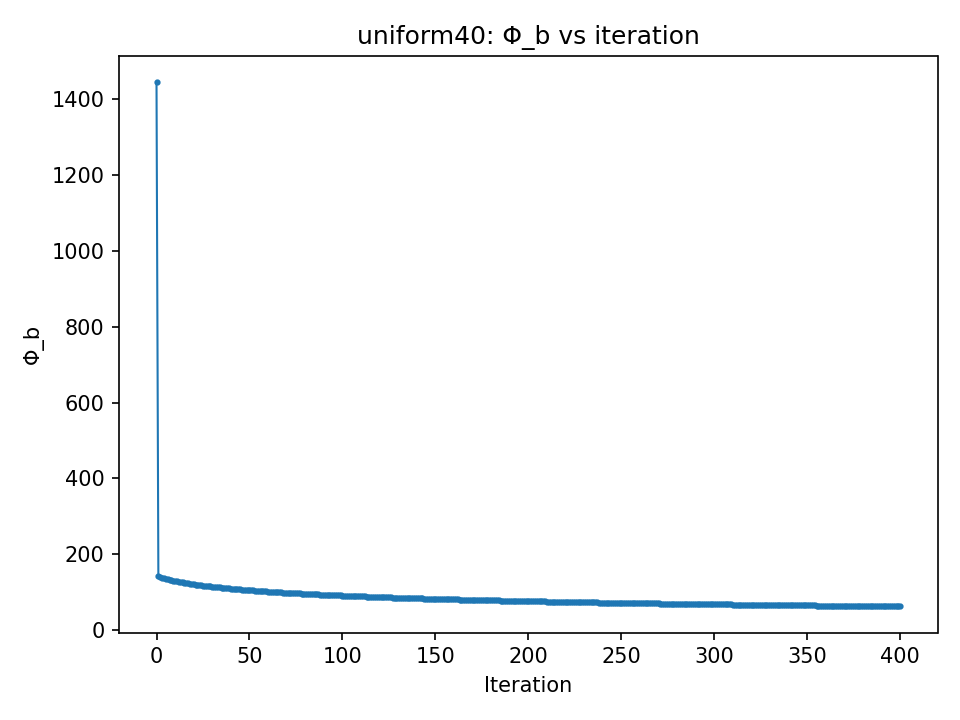
\includegraphics[width=0.32\linewidth]{figures/uniform40_dx0.01_phib_vs_iter.png}
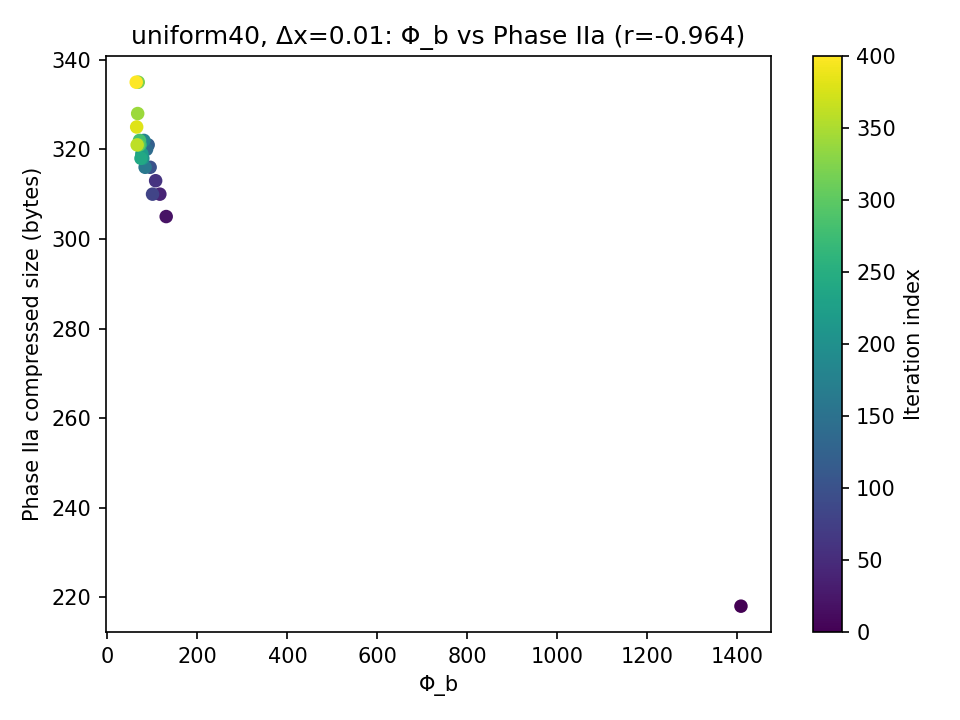
\includegraphics[width=0.32\linewidth]{figures/uniform40_dx0.01_phib_vs_phase2a.png}
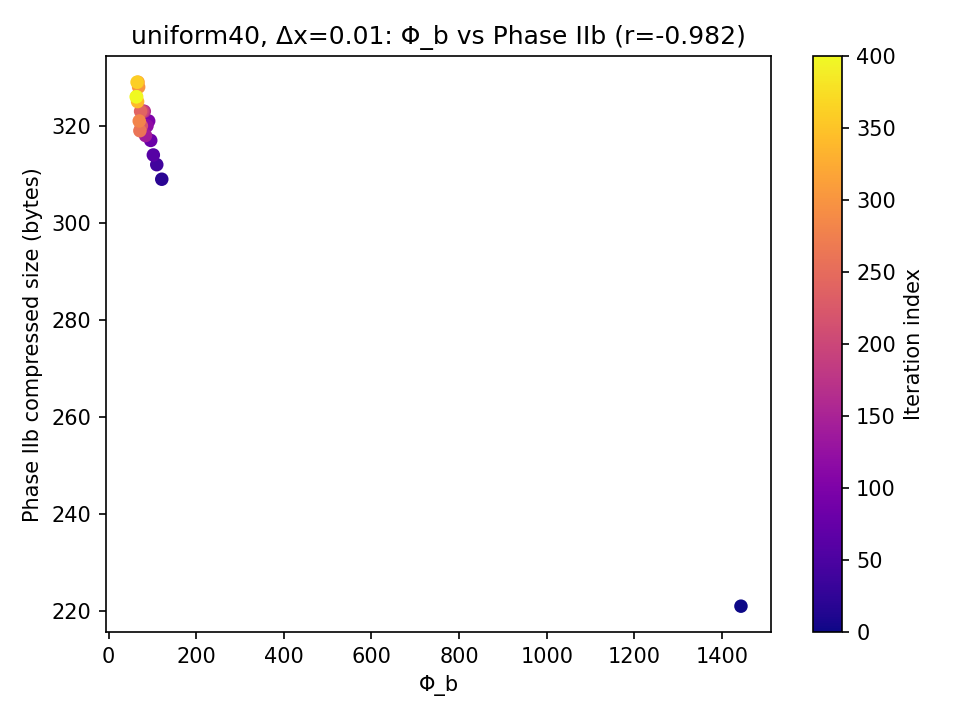
\includegraphics[width=0.32\linewidth]{figures/uniform40_dx0.01_phib_vs_phase2b.png}
\caption{\texttt{uniform40}, $\Delta x{=}10^{-2}$. Left: $\phib$ vs.\ iteration, showing enforced monotone descent (backtracking line search prevents increases). Middle: Phase IIa (fixed-order coordinates $+$ gzip) compressed bytecount vs.\ $\phib$. Right: Phase IIb (random-order coordinates $+$ gzip) vs.\ $\phib$. Strong linear trends persist under ordering control.}
\label{fig:uniform40}
\end{figure}

\subsection*{\texttt{lattice40} ($N{=}40$, $\Delta x = 10^{-2}$)}
\begin{figure}[htbp]
\centering
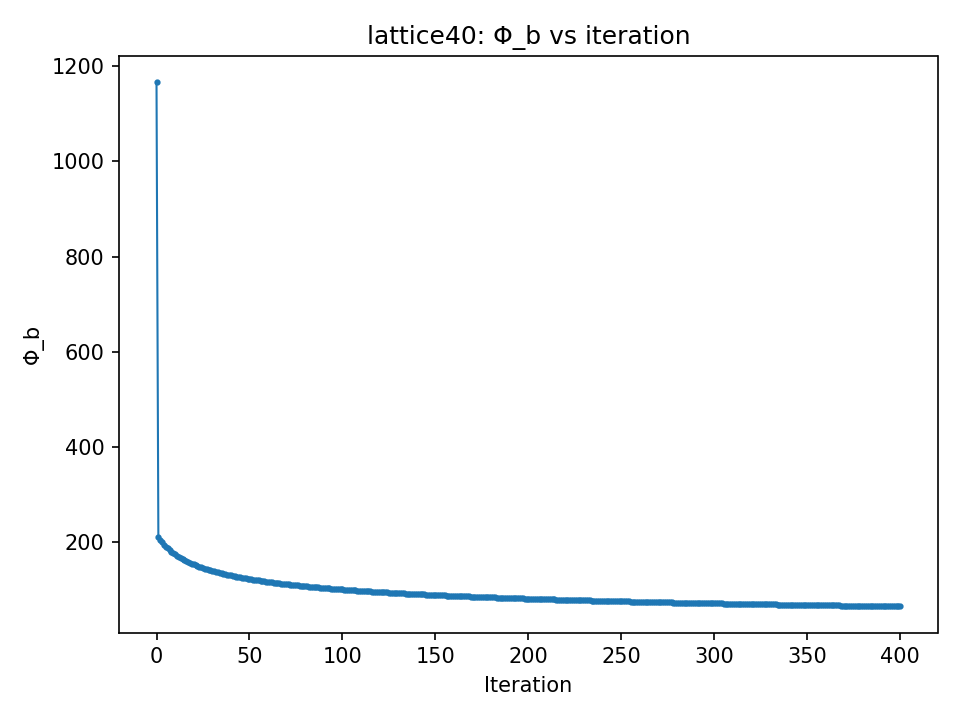
\includegraphics[width=0.32\linewidth]{figures/lattice40_dx0.01_phib_vs_iter.png}
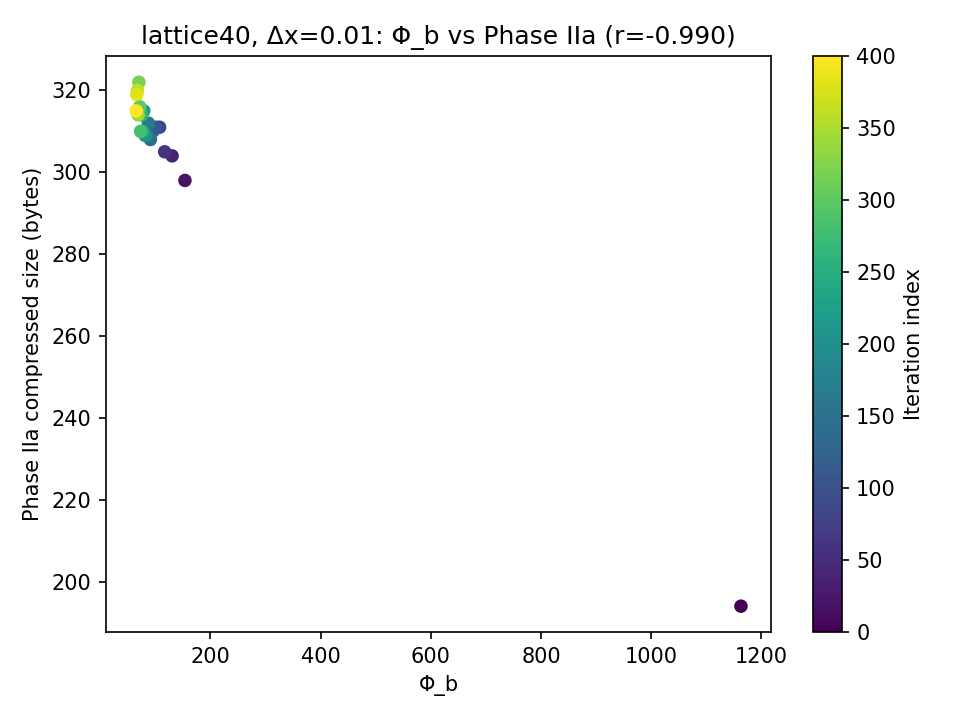
\includegraphics[width=0.32\linewidth]{figures/lattice40_dx0.01_phib_vs_phase2a.png}
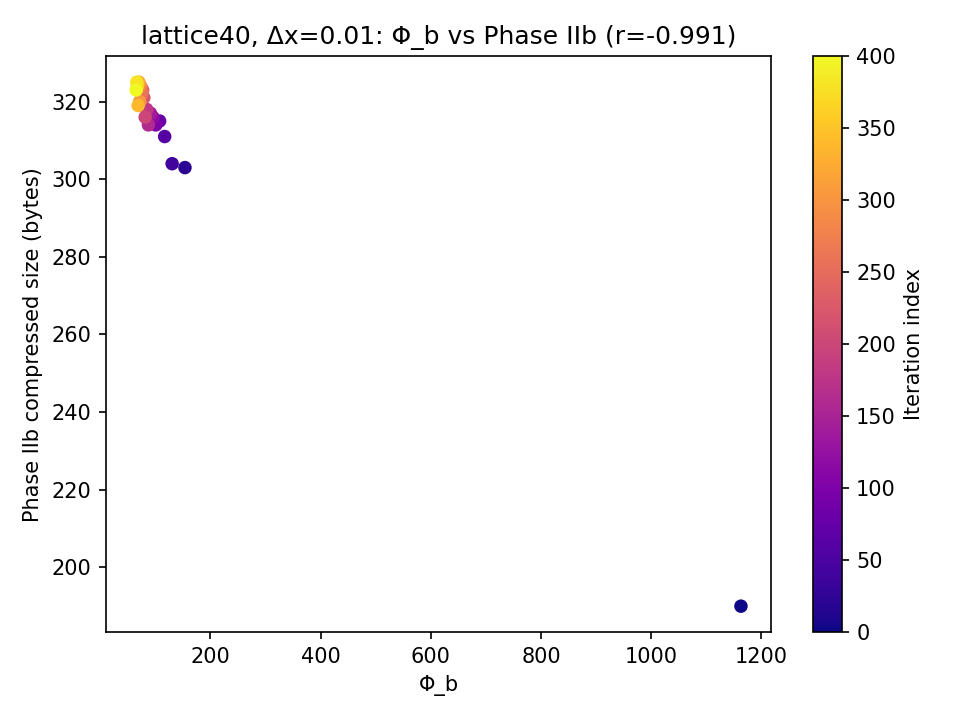
\includegraphics[width=0.32\linewidth]{figures/lattice40_dx0.01_phib_vs_phase2b.png}
\caption{\texttt{lattice40}, $\Delta x{=}10^{-2}$. Left: $\phib$ vs.\ iteration. Plateaus and tiny steps reflect that the initial configuration is already highly ordered, so $\phib$ changes little. Middle/right: compressed bytecount vs.\ $\phib$ under Phase IIa / IIb. Dynamic range is narrow, and $r$ falls below the preregistered $|r|\ge0.7$ bar for some quantizations. F3 therefore flags \texttt{lattice40} as a rejection case.}
\label{fig:lattice40}
\end{figure}

\subsection*{\texttt{blobs40} ($N{=}40$, $\Delta x = 10^{-2}$)}
\begin{figure}[htbp]
\centering
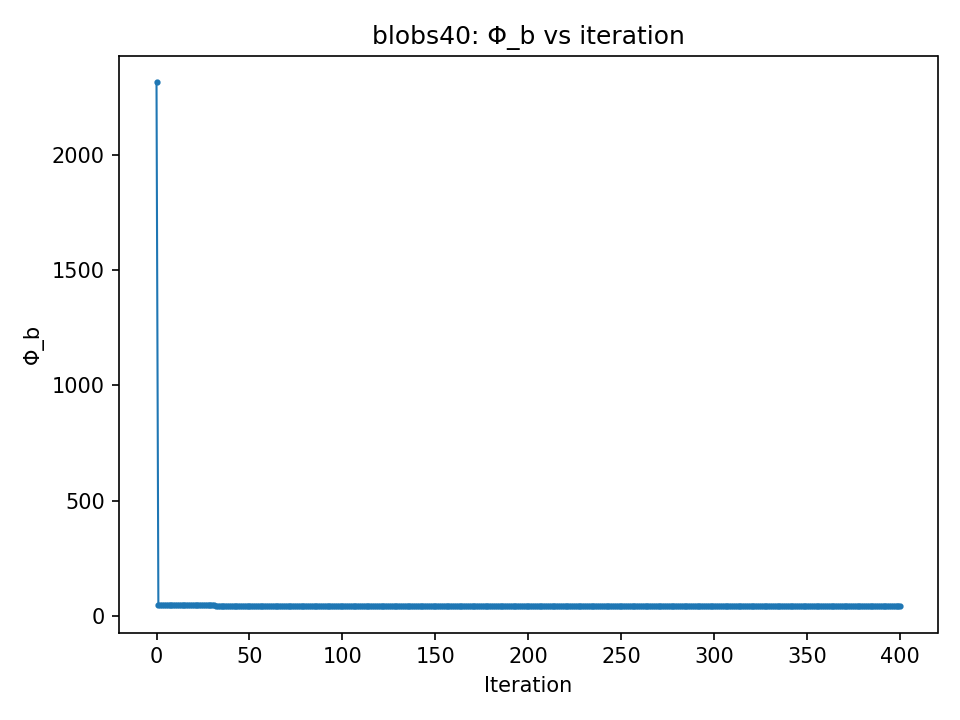
\includegraphics[width=0.32\linewidth]{figures/blobs40_dx0.01_phib_vs_iter.png}
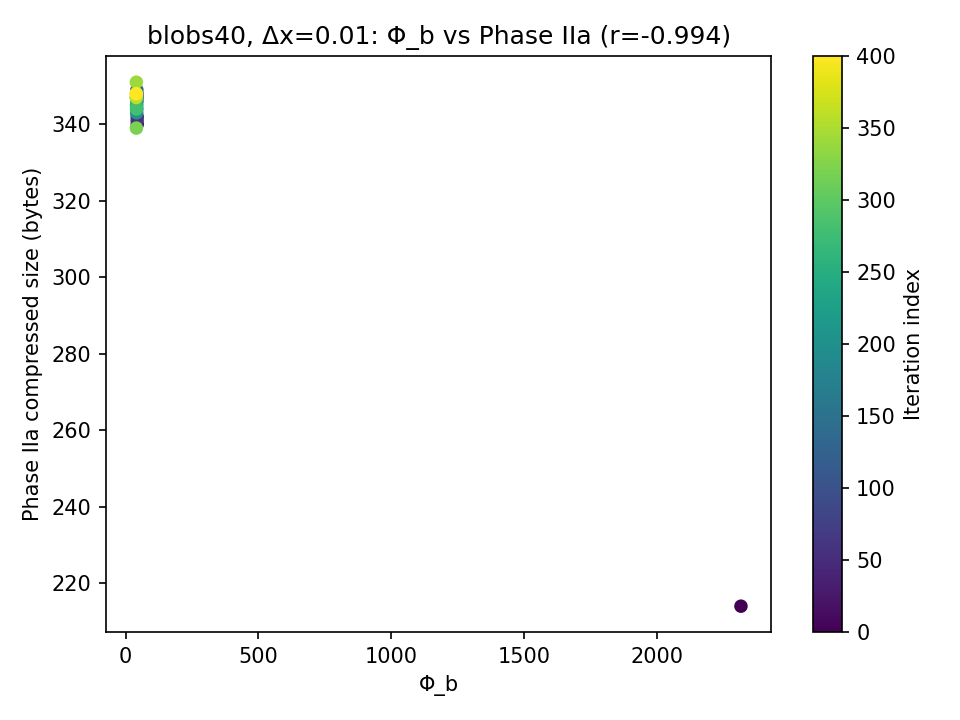
\includegraphics[width=0.32\linewidth]{figures/blobs40_dx0.01_phib_vs_phase2a.png}
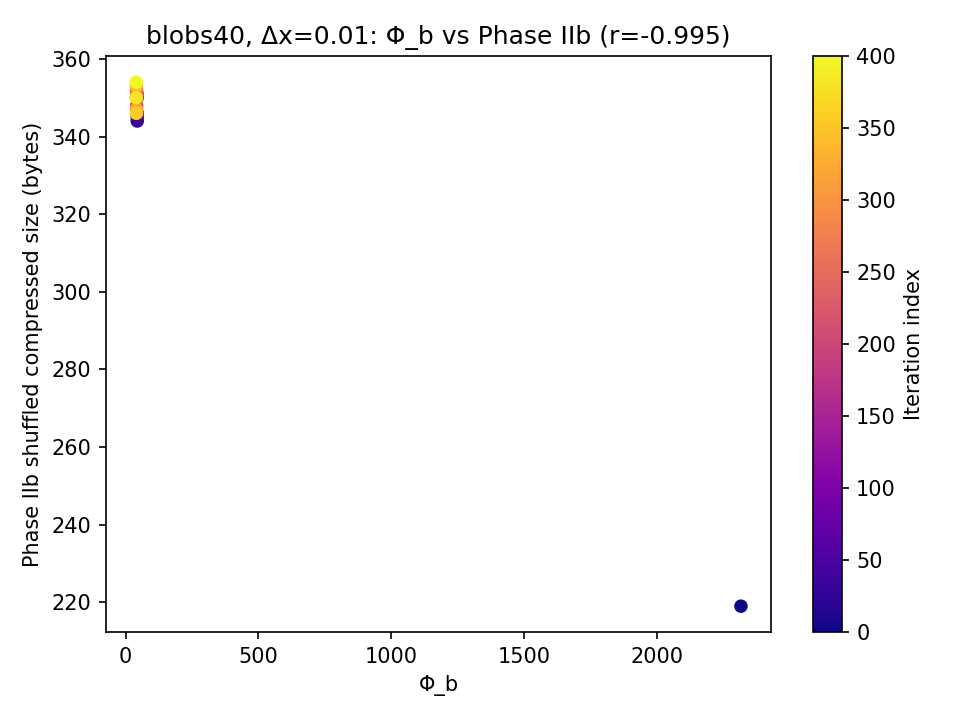
\includegraphics[width=0.32\linewidth]{figures/blobs40_dx0.01_phib_vs_phase2b.png}
\caption{\texttt{blobs40}, $\Delta x{=}10^{-2}$. Two dense clusters descend toward even tighter internal organization. $\phib$ and gzip bytecount track each other almost perfectly, and this persists under Phase IIb's random ordering control.}
\label{fig:blobs40}
\end{figure}

\subsection*{\texttt{uniform400} ($N{=}400$, $\Delta x = 10^{-3}$)}
\begin{figure}[htbp]
\centering
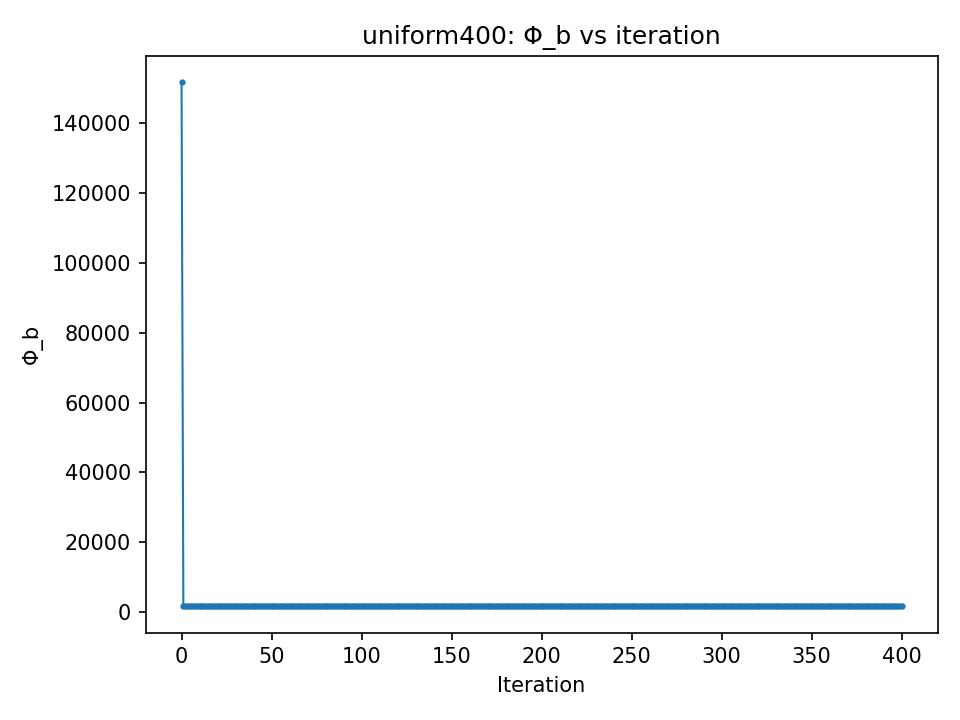
\includegraphics[width=0.32\linewidth]{figures/uniform400_dx0.001_phib_vs_iter.png}
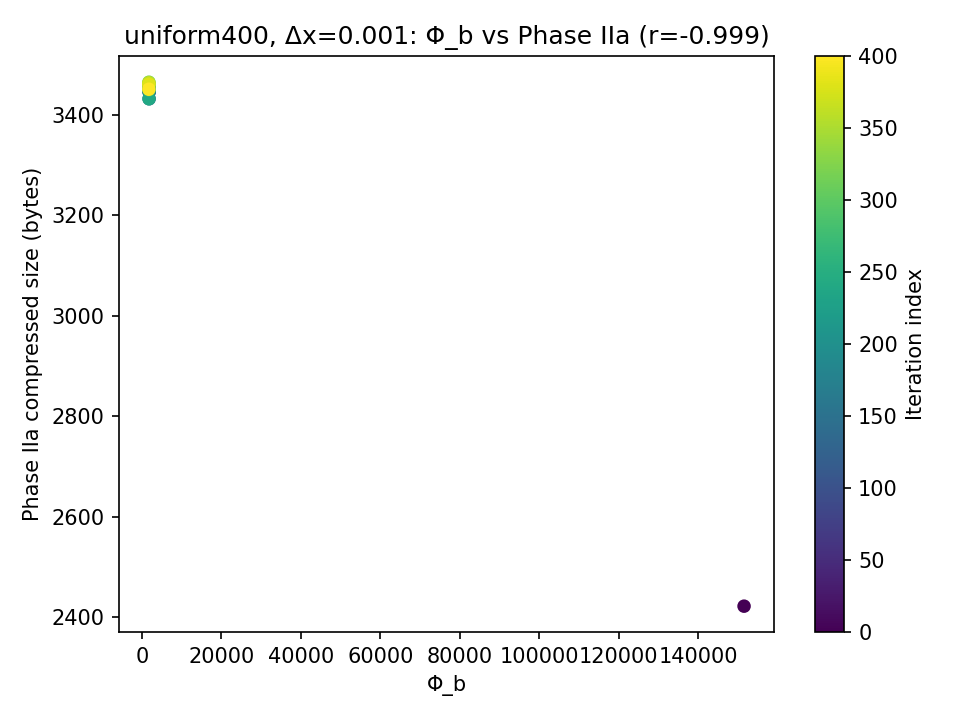
\includegraphics[width=0.32\linewidth]{figures/uniform400_dx0.001_phib_vs_phase2a.png}
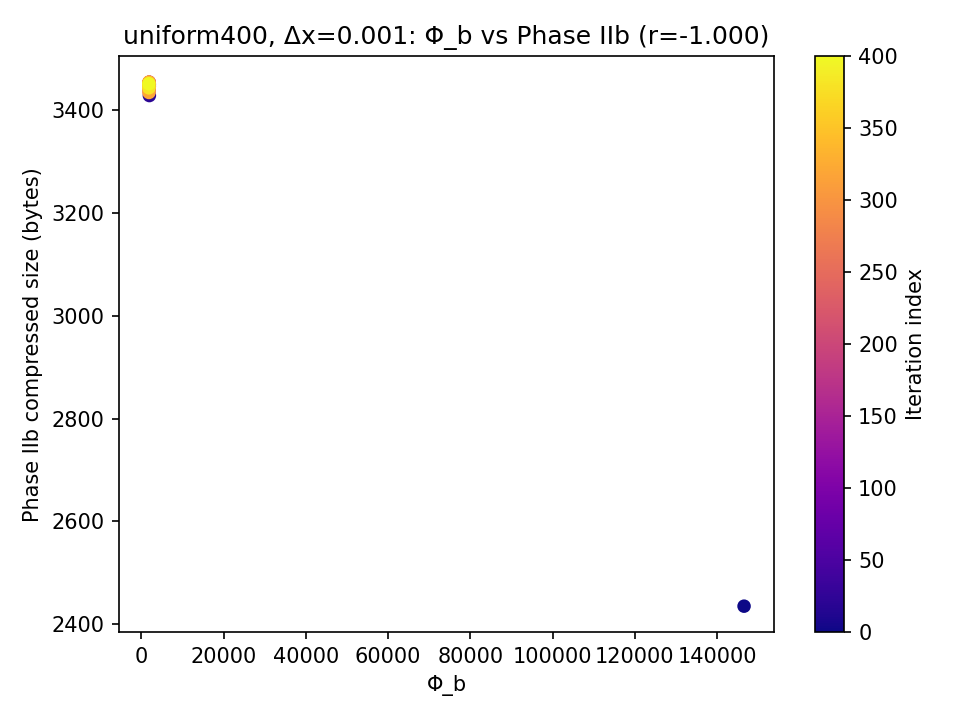
\includegraphics[width=0.32\linewidth]{figures/uniform400_dx0.001_phib_vs_phase2b.png}
\caption{\texttt{uniform400}, $\Delta x{=}10^{-3}$. Even at $N{=}400$, backtracking enforces monotone $\phib$ descent. Correlations between $\phib$ and gzip bytecount approach $|r|\approx 1$ for both fixed-order and shuffled-order coordinate encoders, indicating that large-$N$ structure becomes extremely regular in a way gzip can exploit.}
\label{fig:uniform400}
\end{figure}

\section{Model Card (Preregistered Parameters)}
We regard the following as preregistered for each run:
\begin{itemize}
\item \textbf{System / seed.} $N{=}40$ or $400$ points in $\R^3$, open boundaries, fixed random seed for this pilot.
\item \textbf{Surrogate functional.} $\phib$ in \cref{eq:phib-def} with $a=0.05$.
\item \textbf{Update rule.} Gradient descent with backtracking line search (start $\eta_0{=}0.05$, shrink $0.5$, floor $10^{-6}$); accept only monotone $\phib$ steps.
\item \textbf{Snapshot schedule.} Save every $5$ accepted steps.
\item \textbf{Quantization.} $\Delta x \in \{10^{-1},10^{-2},10^{-3}\}$.
\item \textbf{Encoders.} Phase I (pair-distance histogram $+$ gzip); Phase IIa (fixed-order quantized coords $+$ gzip); Phase IIb (random-order coords $+$ gzip).
\item \textbf{Baselines.} Radius of gyration $R_g$, nearest-neighbor distance, and coordinate variance.
\item \textbf{Subsampling / $n_{\text{eff}}$.} Keep every 20th saved snapshot to reduce autocorrelation, yielding $n_{\text{eff}}\approx 21$ per ensemble.
\item \textbf{Falsifier.} F3 rejects $\phib$ for an ensemble if no encoder at any $\Delta x$ reaches $|r|\ge0.7$ on the decorrelated subsample.
\end{itemize}

\section{Limitations and Next Steps}
\subsection*{Statistical power and replication}
Each ensemble here is a \emph{single} random seed with $n_{\text{eff}}\!\approx\!21$ subsampled snapshots. Pearson $r$ at $n{\sim}20$ is an \emph{effect-size indicator}, not a population estimate. We do not attach $p$-values or CIs. The intended Phase II study is to run 50+ seeds per ensemble, compute bootstrap confidence intervals on $r$, and report distributions of $|r|$ across seeds.

\subsection*{Compressor scope}
gzip is treated as a fixed external encoder that measures byte-pattern redundancy after quantization. It is not assumed to approximate Shannon entropy. Future work will add bzip2, zstd, LZMA, and uncompressed-size controls to test whether the relationship depends on the specific compressor.

\subsection*{Causality / out-of-distribution}
This pilot measures self-consistency along $\phib$-driven descent: we evolve \emph{by} $\phib$, and we ask whether $\phib$ tracks gzip bytecount along that very trajectory. A stronger causal claim would require testing $\phib$ on states \emph{not} produced by $\phib$ (e.g.\ equilibria of other potentials, turbulent flows). That out-of-distribution test is future work.

\subsection*{Alternative surrogates}
Here we tested one softened pairwise surrogate $\phib$. PCD is designed to audit \emph{any} computable surrogate. Phase II will compare multiple surrogates (e.g.\ exponential kernels, Lennard--Jones, Gaussian RBF) under identical encoders and falsifier F3.

\subsection*{Threshold rationale}
The heuristic $|r|\ge0.7$ bar in F3 is meant to flag ``strong linear link'' in this pilot. Observed values naturally separate into $|r|\approx 1$ (clear passes) and $|r|<0.8$ (borderline/fail). In future replicated studies we will set this threshold using the distribution of $r$ across seeds and bootstrap CIs.

\subsection*{Scaling}
At $N{=}400$, correlations approach $|r|\approx 1$ even under Phase IIb (randomized particle order). We interpret this as large-$N$ structure becoming dramatically more regular in a way gzip exploits. Larger $N$ and multi-seed sweeps will test whether this trend is robust or an artifact of a single initialization.

\section{Relation to Prior Work}
This work sits at the interface of:
\begin{itemize}
\item \textbf{Gradient flows / force-directed methods.} We literally descend a scalar potential to drive organization.
\item \textbf{Compression / MDL heuristics.} We treat gzip-compressed bytecount as an external, fixed code length.
\item \textbf{Preregistration / falsifiability.} We define a falsifier (F3), execute it, and keep runs that ``fail'' (e.g.\ \texttt{lattice40}).
\end{itemize}
The point is not that $\phib$ is ``true.'' The point is that we can specify, audit, and \emph{reject} a proposed surrogate in a transparent, reproducible loop.

\section{Conclusion}
PCD provides a minimal reproducible loop:
\begin{enumerate}
\item choose a computable surrogate $\phib$;
\item evolve a system by monotone descent in $\phib$;
\item record gzip-based and histogram-based bytecounts at snapshots;
\item sweep quantization $\Delta x$ and compare to cheap baselines;
\item compute $r$ on decorrelated subsamples and apply F3;
\item record which ensembles are provisionally supported and which are rejected.
\end{enumerate}

In this pilot, three ensembles exhibit near-perfect co-movement between $\phib$ and gzip-based bytecount under both fixed-order and shuffled-order encoders, across three orders of magnitude in $\Delta x$. One ensemble is explicitly rejected. The workflow therefore (i) produces strong effect sizes where present, (ii) reports rejections where not, and (iii) exposes its statistical limits in full view. Phase II is replication and extension, not invention.

\section*{Acknowledgments}
We thank colleagues and reviewers for insisting on ordering controls (Phase IIb), quantization sweeps, geometric baselines, temporal subsampling, and explicit preregistration of the falsifier. Any remaining eccentricities are the author's own.

\bibliographystyle{plain}
\begin{thebibliography}{10}

\bibitem{Shannon1948}
C.~E.~Shannon.
\newblock A mathematical theory of communication.
\newblock {\em Bell System Technical Journal}, 27:379--423, 623--656, 1948.

\bibitem{Rissanen1978}
J.~Rissanen.
\newblock Modeling by shortest data description.
\newblock {\em Automatica}, 14(5):465--471, 1978.

\bibitem{LeimkuhlerMatthews2016}
B.~Leimkuhler and C.~Matthews.
\newblock {\em Molecular Dynamics}.
\newblock Springer, 2016.

\bibitem{FruchtermanReingold1991}
T.~M.~J. Fruchterman and E.~M. Reingold.
\newblock Graph drawing by force-directed placement.
\newblock {\em Software: Practice and Experience}, 21(11):1129--1164, 1991.

\end{thebibliography}

\end{document}
